\section{Proposed architechture}
\label{sec:propesedArch}

\quad The HBlast architecture, proposed in this paper, was designed for small query (512-bit = 256 letter) but for large sized data base (4GB).  First, database sequence will be saved in double data rate(DDR) SDRAM and query sequence will be saved in register \textit{queryReg}. Then the actual alignment operation will start. 
   
\begin{figure}[h!]
\centering
\includegraphics[width=\columnwidth]{Figures/BlastMachine.pdf}
\caption{Proposed Architecture / HBlast machine.} \label{fig:blastArch}
\end{figure}

The two main blocks of the HBlast architecture are \textit{Hit} and \textit{Expand}, while \textit{Memory Interface} acts as a control logic for them, refer to \textit{Fig.\ref{fig:blastArch}}. As their names state, these blocks are responsible for tasks like finding hit (match), expanding the sequence and linking blocks. 

For the nucleotide W-mer size is 11 letters, so by \textit{Eq.\ref{eq1}} there are 246 W-mers in 256-letter query. Each of them must be compared with one W-mer of the database.  Comparison of one database and one query W-mer at a time is not effective in terms of timing. In HBlast architecture this operation is parallelized by introducing 246 comparators (one for each query W-mer). All comparators have one common input: 22-bit (11-letter) database W-mer. This input is controlled by \textit{Database Shift Register}, which perform 2-bit shift after each iteration. The expansion will start if output of any of these comparators is high. 



The expansion and hit are sequential operations not parallel, meaning that the expansion will start only if the hit stops and other way around. After the hit operation finishes, it will send information about the location of the match in query and number of performed shift operations. Loading the data from memory interface is controlled by signal \textit{load}. The number of state changes of the signal (low or high) is then decided by examining \textit{shiftNumber}. There can be at most two read operations for one iteration. Each time the read data will be saved in 512-bit \textit{Database} register and then merged into 1024-bit register, \textit{MergedDatabase}. Then the expansion will work by the logic described in the following \textit{Expand Finite State Machine} section. 
At the same time the block \textit{High Score Calculator} will calculate the match score and keep track of the five HSP (with their location in database and query).    



\subsection{Hit}
\quad Hit (hit.v module) is one of the two main modules in proposed architecture, which is aimed to compare W-mers from the database with W-mers in query in parallel and to find exact match. The module is a finite state machine (FSM) of two states, refer to \textit{Fig.\ref{fig:hitFSM}}. In the first state (\textit{Idle state}), the module takes 22 bits of sequence from the database and compares the W-mer with each W-mer from the query sequence via 246 comparators. Parallel architecture of FPGA allows performing the task simultaneously, which significantly improves timing. Then, if at least one exact match is detected, the signal \textit{hit} is received and the process passes to the next state, (\textit{HitLow}).It stays in this state while expansion process is being performed. When expansion is over, the process again goes to \textit{Idle state} and verifies if there are other matches of the W-mer within the query. If there is a match again, the expansion process will be repeated, if there is no more match found, the loaded 512 bits of database is shifted by 2 bits and next 22 bits of sequence in database are gone through all the processes described above. When all W-mers in the database are compared, then next 512 bits of the database are loaded and process is initiated again. 

\begin{figure}[h!]
\centering
\includegraphics[width=\columnwidth]{Figures/hitFSM.pdf}
\caption{FSM diagram for module Hit} \label{fig:hitFSM}
\end{figure}



\subsection{Expansion Finite State Machine}
\quad Expansion Finite State Machine (ExpansionFSM.v module) is a second main module that expands exactly matched sequence of the database to both sides by comparing it with the query. The outputs of the module are start and end locations of the expanded matching sequence and its high score. Expand FSM is a FSM of 6 states, refer to \textit{Fig.\ref{fig:expandFSM}}:

\begin{enumerate}
  \item \textbf{Idle}: It stays in in this state until the signal that indicates the start of the expansion comes.
  \item \textbf{Wait}: In this state module waits until the signal of loading data from DDR is received. 
  \item \textbf{Load 1}: This state loads the 512-bit piece of database to register. Then it passes to the next state according to the shift number by following logic: if the shift number is less than 199 or more than 290, it goes to state \textbf{Load 2}; otherwise it goes to the state \textbf{Expand} directly. . 
  \item \textbf{Load 2}: This state decides to take another 512-bit piece of database located either before or after the database with exact matched sequence. The address of the piece is calculated within the state and it goes to the next state which waits loading of the piece. 
  \item \textbf{Merge}: In this state the 512-bit piece of database merges with another 512-bit sequence. This is done in order to broaden expansion's scopes.
  \item \textbf{Expand}: The exactly matched W-mers of database and query expands to both sides by 2 bits each clock.
\end{enumerate}

The initial value of HSP is 55 (obtained from 11*5). If next 2 bits are matched 5 is added to the HSP, otherwise 4 points are subtracted. Threshold value is chosen to be 200 bits, meaning that the sequence can be expanded to both sides by 200 bits each. Accordingly, maximum HSP can be 1055. 
       

\begin{figure}[t!]
\centering
\includegraphics[width=\columnwidth]{Figures/expandFSM.pdf}
\caption{FSM diagram for module Expansion} \label{fig:expandFSM}
\end{figure}
       
       
\subsection{Memory Interface}
\quad The module Memory Interface (memInt.v module) is a control unit that interacts with modules Expansion FSM, Hit and bridge. It is an FSM of 7 states. The main functions of the module are following:
\begin{itemize}
\item The module takes addresses from the expansion or hit modules and loads respective data.
\item Module receives and sends control signals. For instance, when it gets signal which indicates absence or expiration in matches between query and 22-bit W-mer of the database from Hit module, it sends signal to shift the current piece of the database to the module.
\item The module allows to perform the whole process sequentially and to avoid confusion of dataflow between ExpandFSM and Hit modules. For example, the address of the data that must be passed from Hit to ExpandFSM are calculated in the module and are used to load necessary data.
\end{itemize}

\begin{figure}
\centering
\includegraphics[width=\columnwidth]{Figures/FSM_Mem_New.pdf}
\caption{FSM diagram for Memory Interface} \label{fig:MemInt}
\end{figure}


\subsection{Bridge}
\quad The Bridge module is the module which makes data width matching between FPGA board with 7 series Memory Interface. It consists of four states, refer to Fig. xxx:
\begin{enumerate}
\item \textbf{Idle}. Depending on whether input signal is write or read, the state changes to Wait\_wr\_cmd and Wait\_rd respectively. Write signal comes from PCIe when it wants to write query data and database into DDR SDRAM. While, read signal comes from two main modules (Hit and Expand) of the architecture when it wants to take data from DDR.
\item \textbf{Wait\_wr\_cmd}. This state waits for the acknowledgement from DDR, as it is received, input data is sent to DDR. Then, state changes to the next Wait\_wr state.
\item \textbf{Wait\_wr}. The present state waits for write\_ready acknowledgment, then increments the write address, which is byte addressable, by 8. The reason for this is that each time we write 64 bits of data, which is 8 bytes. For instance, in order to write 512-bit sequence, 8 writes are needed. After all these operations, it goes to Idle state.
\item \textbf{Wait\_rd}. After receiving acknowledgment from DDR that DDR is ready, it reads data for 8 times and each time increments initial address by 8 for the same reason as explained above. After these operation are completed, the state is changed to Idle. 
\end{enumerate}


\begin{figure}
\centering
\includegraphics[width=\columnwidth]{Figures/bridgeFSM.pdf}
\caption{FSM diagram for bridge} \label{fig:bridge}
\end{figure}
